\section{Sensorenhet}
Sensorenheten har i uppgift att läsa in sensordata och omvandla den till ett läsligt format. Den innehåller en processor av modellen ATmega1284, flera IR-sensorer, en lasersensor, samt gyro.

IR-sensorerna används primärt för navigering, så att roboten kan köra i en rak linje längs en vägg. Lasersensorn används för skanning av rummet. Med hjälp av gyrot går det att hålla koll på robotens rotation.
Se figur \ref{fig:unitSensor} för en övergripande systemskiss för sensorenheten.

\begin{figure}[h!]
	\makebox[\textwidth][c]{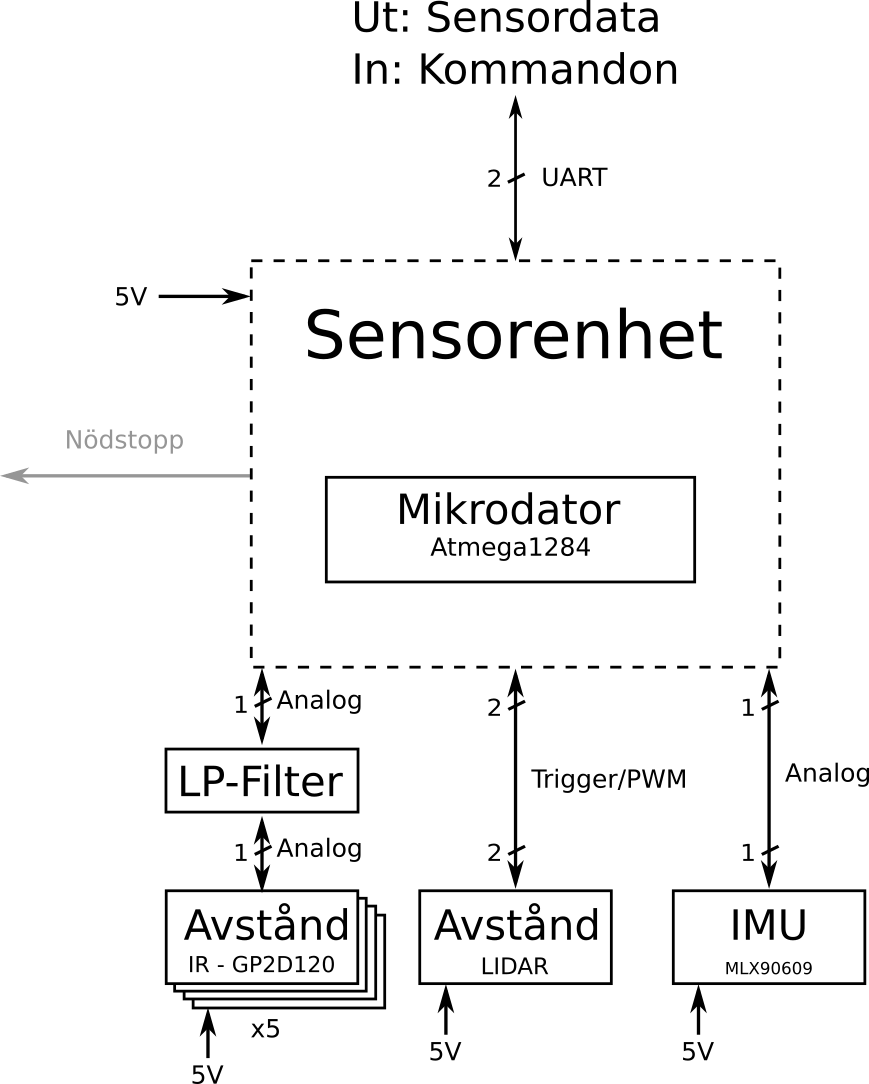
\includegraphics[width=0.6\textwidth]{sensorenhet.png}}
	\caption{Översikt över sensorenheten.}
	\label{fig:unitSensor}
\end{figure}

\subsection{Hårdvara}

\subsubsection{Processor}
ATmega1284 används som processormodell, då den är kraftfull utan att ta det till överdrift. Antalet pinnar, A/D-omvandlare, interrups samt UART-enheter som processorn har räcker för samtliga sensorer och kommunikationsbussar.

\subsubsection{IR-sensorer} \label{sssec:sonicsensors}
Det placeras två stycken IR-sensorer av modell GP2D120 på både höger och vänster sida om roboten (för totalt fyra), samt en på baksidan. För avståndsmätning framåt används LIDARn. Dessa sensorer används för navigering och positionsuppskattning. Med hjälp av de dubbla IR-sensorerna på vardera sida kan det avgöras ifall roboten åker parallelt med väggen. Dessa behöver en A/D-omvanlare var, som är inbyggd i processorn ATmega1284. Se kapitel \ref{ssec:sensorInterface}. Sensorerna kan effektivt mäta avstånd inom intervallet 4 till 30 cm vilket räcker, då roboten är tänkt att följa en vägg och köra inom ett rutnät på 40x40cm.

\subsubsection{LIDAR lite v2} \label{sssec:lidar}
LIDAR Lite v2 är en lasersensor som används för mätningar som kräver bättre noggranhet. Komponenten kommunicerar via en trigger-pin och PWM-output.

LIDARn används också som en sensor framåt, för attt avgöra ifall robotten kan fortsätta att köra.

Sensorn monteras på toppen av roboten - ovanpå ett roterande servo, som specificeras i större detalj i kapitel \ref{ssec:servomotor}. Detta för att kunna mäta avstånd i flera vinklar utan att snurra roboten.

\subsubsection{Gyro} \label{sssec:imu}
MLX90609 är ett gyro som används via en analog ingång. Den ger oss rotationen kring z-axeln, som användas för att beräkna robotens riktning i rummet under svängar.
Gyrot läses endast av när det efterfrågas (under sväng).

\subsubsection{Komponentbudget}
Här följer en lista på all hårdvara som detta delsystem kräver.

%TODO Uncomment after rebase; hardware list is not yet defined in LIPS.tex
%\begin{HardwareList}
%\hardware{Atmega1284p}{Mikroprocessor med 44 pinnar (inklusive 8 A/D-omvandlare).}{1} %TODO: Eventuellt LP-filter till AVCC-porten. Finns ej i Anders föreläsning, men i många andra.
%\hardware{IQEXO-3}{Occilator för Atmega-klockan, med standardfrekvens 16MHz}{1}
%\hardware{GP2D120}{IR-sensor.}{5}
%\hardware{Kondensator}{Till LP-filter för IR. Storlek bestäms av frekvensen på störningarna.}{5}
%\hardware{Resistans}{Till LP-filter för IR. Storlek bestäms av frekvensen på störningarna.}{5}
%\hardware{LIDAR lite v2}{Avancerad lasersensor.}{1}
%\hardware{Resistans}{Separation av trigger och monitor för LIDAR. 1k.}{1}
%\hardware{Kondensator}{Störningsreducering av LIDAR. 680uF.}{1}
%\hardware{MLX90609}{Gyro.}{1}
%\hardware{Kondensator}{Störningsreducering av gyro. 1uF. Datablad rekommenderar X5R eller X7R med minsta spänning 10V.}{2}
%\hardware{Kapacistans}{Störningsreducering av gyro. 0.1uF. Datablad rekommenderar X5R eller X7R med minsta spänning 25V.}{1} % TODO: Finns en till typ frivillig, se datablad. Finns inritad i schemat.
%\end{HardwareList}

\subsection{Mjukvara}

Koden skrivs i C, och ska följa standarden specificerad i bilaga \ref{sec:cstandard}.

Programmet omvandlar sensordata till ett mer läsligt format, och skickar det vidare (se kapitel \ref{ssec:sensorInterface}), samt tar emot instruktioner om att läsa av en viss sensor. 

Sensorenheten ska kontinuerligt läsa av sensorerna, på detta sätt går det smidigt att även kolla baklänges på tidigare avläsningar. Att läsa av sensorerna kontinuerligt gör det möjligt för sensormodulen att vara medveten ifall roboten följer en vägg eller inte. Sensorenheten kommer att ha en interrupt, som ger möjligheten för den att läsa av sensorer direkt när en avläsning begärs.

% TODO Avläsningsinstruktioner? Menas kommandon som: ``Tja, jag ser gärna detta avläst''? Bör förtydligas och utvecklas. - Tillräckligt?

% TODO Denna sektionen känns i största allmänhet alldeles för tunn. Utveckla mer. Lägg till flödesscheman.

\subsection{Gränssnitt} \label{ssec:sensorInterface}
Sensorenheten ska kommunicera med alla sensorer och skicka vidare utdata. Sensorenheten tar emot uppmaningar om att starta en avläsning via samma UART-buss som används för att rapportera mätvärden vidare.

% TODO Utveckla den här sektionen. Nämn inte I2C; det används inte. Jag misstänker att det mesta av texten nedan bara är rakt ur systemskissen.

\subsubsection{LIDAR}
LIDAR kommer använda avläsningstriggers och PWM via en gemensam pin på sensorn. På Atmega-sidan delas denna upp i två pinnar med en resistor på triggersignalen som gör att LIDARns signaler får prioritet. PWM-signalen kopplas ett avbrott för att mäta dess längd, som används för att beräkna avståndet.

\subsubsection{Gyro}
MLX90609 stödjer avläsning via en analog pinne samt via SPI. Vi använder analog avläsning. Mätvärdeskalibrering med hjälp av temperatursensorn på gyrot används ej, så länge mätvärdena är noggranna nog för våra behov.

\subsubsection{IR-sensorer}
IR-sensorerna använder en analog utgång som varierar i enlighet med avståndet efter en ickelinjär kurva. Denna signal har störningar som måste filtreras ut med hjälp av LP-filter, se kopplingsschema. Värden på LP-filtret måste beräknas efter mätning av störningarna.

IR-sensorer kommer att genomföra kontinuerligt mätningar för att avgöra ifall roboten åker rakt fram. Det finns också möjlighet till avläsningstriggers, så att när det kommer en begäran om avläsning kan detta genomföras ögonblickligen.

\subsubsection{Utvärden/Input}
En UART-buss via den inbyggda UART-hårdvaran används. Via denna buss tas avläsningsinstruktioner emot och sensordata skickas.

\newpage